\section{Introduction}

Humans actively use vision during everyday activities to gather and refine information about the environment. Since the seminal works of \citet{Yarbus2013-eu} and \citet{Buswell1935-di} there has been consistent evidence that eye movements depend on the viewing task the observer is performing.  \citet{Kollmorgen2010-wg} demonstrated stimulus dependent features, spatial viewing biases and task dependent features all influence the exploration of a visual scene. This is further supported by studies that emphasize the relevance of semantics in guidance of eye movements \citep{Henderson2017-it, Einhauser2008-yi}. Thus, we have growing evidence that task demands can affect eye movements behavior.

In a pragmatic turn in cognitive science, there is a greater push towards incorporating the study of cognitive processes while interacting with the external world \citep{Parada2020-qq}. Moreover, \citet{Engel2013-bx} proposed that cognition encompasses the body and in turn, bodily action can be used to infer cognition. To this effect, understanding the control of eye movements in natural, real-life situations requires a mobile setup that allows for a subject to be recorded in tandem with volitional actions in a controlled yet unconstrained environment. Studying eye movements in mobile subjects might give us a richer picture of cognitive processing in more naturalistic settings.

Seminal studies have already investigated eye movement behavior in natural environment with fully mobile participants. In the pioneering studies of \citet{Land1999-ol} and \citet{Hayhoe2003-lw}, subjects performed everyday activities of tea-making and sandwich-making, respectively. These studies required a sequence of actions which involved manipulating objects one at a time to achieve the goal. Both studies showed that nearly all the fixations were task-related. Further studies investigated eye movements under a plethora of natural condition while walking \citep{Matthis2018-ho}, driving \citep{Mars2012-bn, Sullivan2012-gg, Navarro2020-wv}, hand-washing \citep{Pelz2001-cn}, hitting a ball \citep{Land2000-pw}, and free exploration \citep{Schumann2008-un}. These experiments in naturalistic settings have revealed several distinct functions of the eye movements during habitual everyday tasks.

These studies uncovered a systematic timing of visual fixations and object manipulation. Specifically, fixations are made to target objects about 600ms before manipulation. More importantly, \citet{Ballard1995-ji} proposed a "just-in-time" strategy that universally applies to this relative timing of fixations and actions. In other words, fixations that provide information for a particular action immediately precede that action and are crucial for a fast and economical execution of the task

While performing habitual tasks fixations can be broadly categorized into four functional groups \citep{Land2001-do}. ’Locating’ fixations retrieve visual information. ’Directing’ fixations acquire the position information of an object and accompany a manipulation action and facilitate reaching movements. ’Guiding’ fixations alternate between two objects being manipulated e.g., knife, bread, and butter. ’Checking’ fixations monitor where the task constraints in the scene have been met. These findings have also been corroborated by \citet{Pelz2001-cn} and \citet{Mennie2007-my}. \citet{Pelz2001-cn} showed similar just-in-time strategy of gaze allocation while performing a hand-washing task. They also reported a small number of fixations of about 5\% that did not serve the immediate sub-task but rather provided information that would be needed for a future action. The authors hypothesize these ´Look-ahead´ fixations provide a mechanism to stabilize the visual input stream that result from a sequence of actions, facilitate task-switching, and reduce conscious effort required to complete the actions in a sequence. Hence, look-ahead fixations can be explained as a perceptual strategy to ease the cognitive load attending to complex tasks in the real world. In sum, the wide-ranging functions of eye movements are well documented in natural routine tasks.

Based on these observations \citet{Land2001-do} proposed a framework that outlines that flow of visual and motor control during task execution \textcolor{Blue}{Figure \ref{figure:task}A}. The process summarizes the various operations that \textit{must} occur during an ’object-related action’ i.e., individual actions performed on separate objects to achieve the desired goal. Each schema "specifies the object to be dealt with, the action to be performed on it, and the monitoring required to establish that the action has been satisfactorily completed." \citep{Land2006-da}. Further, the gaze control samples the information about the location and identity of the object and directs the hands to it. Subsequently, the motor control system of the arms and hands implement the desired actions. Here, vision provides the information of where to direct the body, which state to monitor, and determine when the action must be terminated. Taken together, a ’script’ of instructions is sequentially implemented where the eye movements earmark the task-relevant locations in the environment that demand attentional resources for that action

This matches the common theme in the above studies investigating natural tasks (e.g., tea-making, sandwich-making, hand-washing) with an organized and well-known structure. These tasks involve specific object-related actions such as picking up the knife, picking up the teapot, etc. and have a predefined ’script’ for the execution of the tasks. The studies, therefore, study eye movements that are under strict control of a task sequence. Moreover, these tasks are over-learned and over-generalized as they are part of a habitual action repertoire for an adult human being. As discussed by \citet{Land2006-da} the low-level schemas (locating, directing, guiding, monitoring) defined above are likely not executed under deliberate conscious control. This distinction corresponds to \citet{James2007-zv} distinction between "ideo-motor" and "willed" acts. As James described, ideo-motor actions correspond to movements where we are "aware of nothing between the conception and execution" of the said action. In contrast, the willed actions require "an additional conscious element in the shape of a fiat, mandate, or expressed consent." Hence, it is unclear whether these low-level schemas of gaze control operate similarly for deliberate actions where an internal task script is not already known.

\begin{figure}[H]
    \centering
    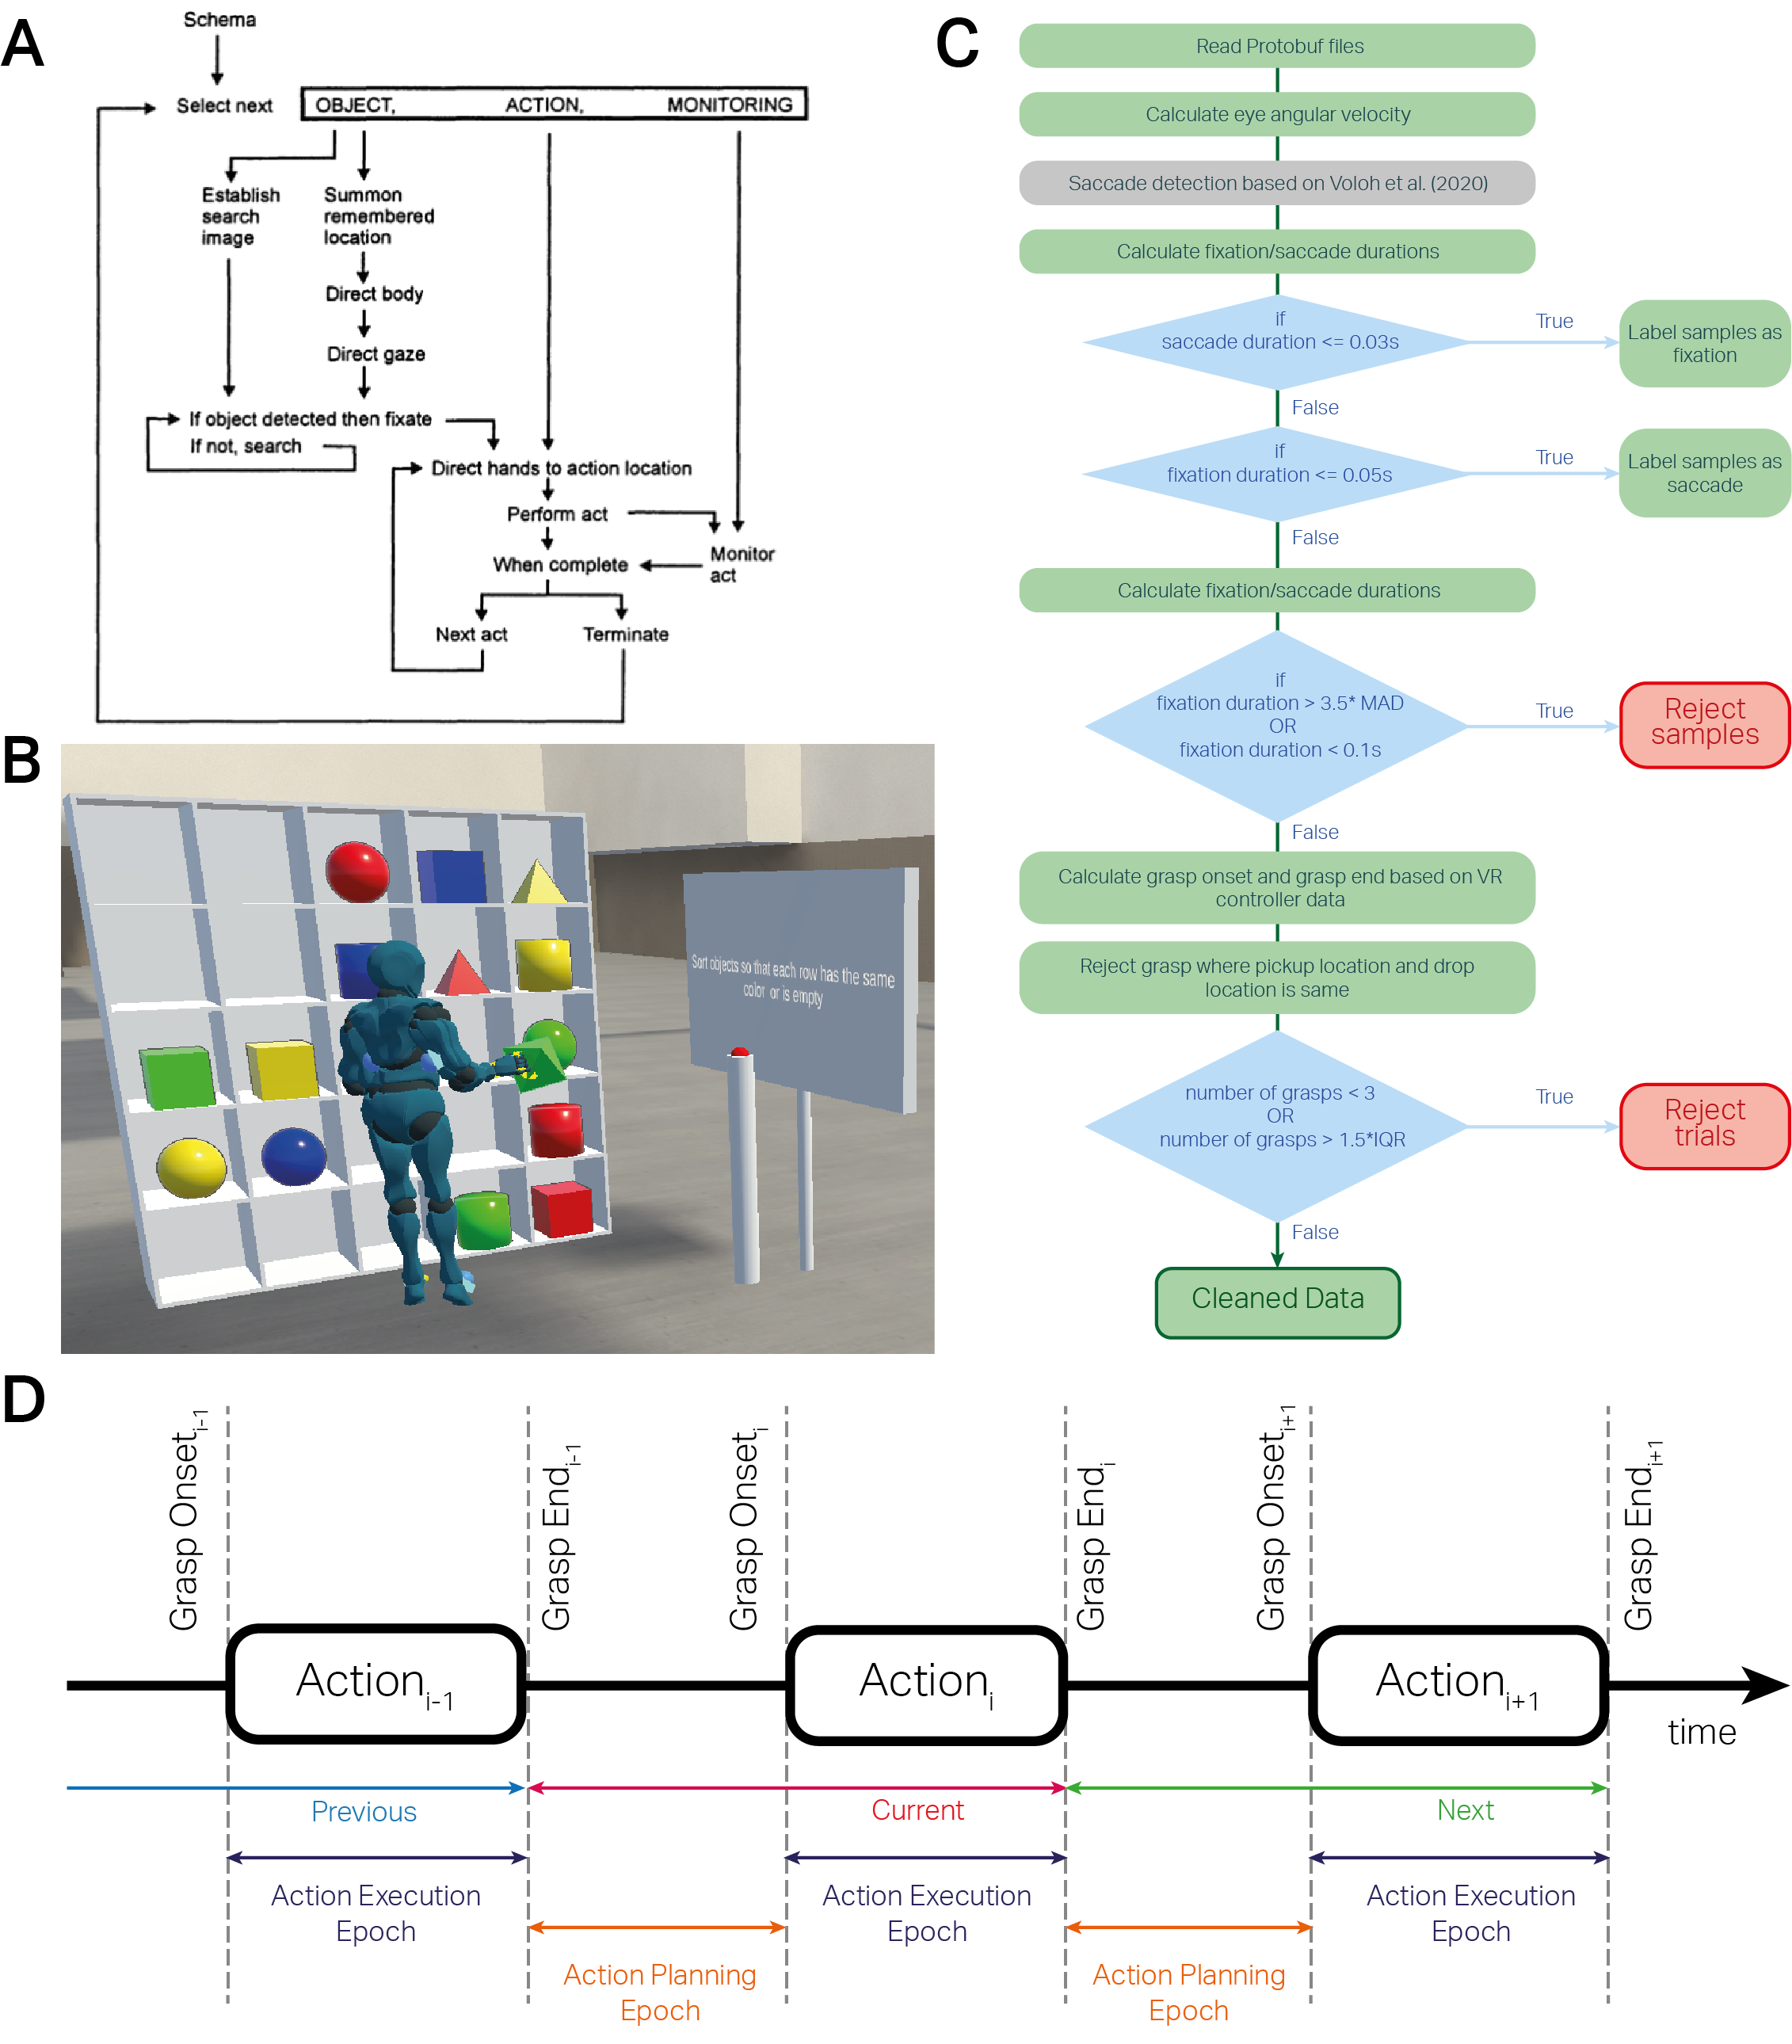
\includegraphics[width=1\linewidth]{source/figures/experiment_setup/Methods_1.png} \\
    \caption[]{\textbf{A.} Schematic of motor and gaze control during performance of natural tasks \citet{Land2001-do}. \textbf{B.} Experimental Task. In a virtual environment participants sorted 16 different objects based on 2 features color or shape while we measured their eye and body movements. The objects were randomly presented on a 5x5 shelf at the beginning of each trial and were cued to sort objects by shape and/or color. Trials where objects were sorted based on just one object feature (color or shape) were categorized as EASY trials. Conversely, in the trials where sorting was based on both features (color and shape) were categorized as HARD trials. All participants performed 24 trials in total (16 easy trials and 8 hard trials) with no time limit. \textbf{C.} Data preprocessing steps for fixation/saccade detection and data rejection. \textbf{D.} Action execution and planning epochs. In order to study the function of eye movements we divided each trial into action planning and action execution epochs. The action execution epochs start from grasp onset till grasp end for each object displacement, whereas the action planning epochs start from grasp end of previous object displacement and grasp onset of current object displacement.}
    \label{figure:task}
\end{figure}

\citet{Norman1986-qb} proposed a theoretical framework for the components of attentional mechanisms that govern deliberate/planned actions. In comparison to the low-level schema proposed by \citet{Land2006-da}, which can account for routine, well-learned tasks, the \citet{Norman1986-qb} model suggests another supervisory module that selects a schema to implement. In well-learned tasks, a schema is triggered automatically without conscious control. However, when a task is fairly complex and requires planning, multiple low-level schemas might compete for resources at the same time and require contention scheduling. For example, contentions can arise on whether to monitor the current action with respect to previous actions or future planned actions to fulfill the task-relevant goals. Such a scheduling mechanism is then required to provide conflict resolution for potentially relevant schemas either by inhibition or activation. Taken together, the model predicts that a failure of the supervisory control can lead to an instability of attention and heightened distraction.

To generalize the above oculomotor behaviors, one could examine the spatial temporal profiles of the fixation in novel task scenarios. First, in cognitively complex tasks an abundance of look-ahead saccades would give evidence of elaborate cognitive planning. That is, high-level planning processes with matching eye movements would also support optimal decision making. Second, the concurrence of cognitive processing and actions would emphasize a strict sequence of fixations with specific purposes, e.g., locating, directing, guiding, checking where cognitive schemas and actions would evolve in parallel. Experiments with complex, variable tasks are needed to differentiate these hypotheses. 

To further pursue this line of research, it is desirable to perform such experiments under tightly controlled laboratory conditions. In recent years, virtual reality (VR) and mobile sensing has offered great opportunity to create controlled, natural environments. Here, subjects’ eye and body movements can be measured reliably along with their interactions with the environment \citep{Keshava2020-cp,Keshava2021-ei, Clay2019-cu, Mann2019-ls}. Experiments in virtual environments have grown popular in recent years and have shown promise towards studying cognition in naturalistic and controlled environments.

In the present study, we investigate the mechanisms of allocation of attention while performing a novel task in a naturalistic environment. We created two types of tasks that varied in complexity and required performing a sequence of actions to accomplish the cued goal. We asked subjects to sort objects on a life-size shelf based on the object features. The complexity of the task depended on sorting based on one object feature or both. We designed the tasks to be novel in a way that subjects had to plan their action sequences on-the-fly and in absence of a pre-defined action "script". We concurrently measured the eye and body movements while subjects performed the tasks.
